\gdef\problemNumber{Not in a book}
\def\problemText{
Given the following graph, use Dijkstra's algorithm to find shortest paths from
vertex A to all other vertices. Indicate the order in which vertices are
selected, and the cost of each selected vertex. After each selection / update,
show the cost and parent of each unselected vertex.\parend
Assume all edge lists are processed in alphabetic order.\\[12pt]
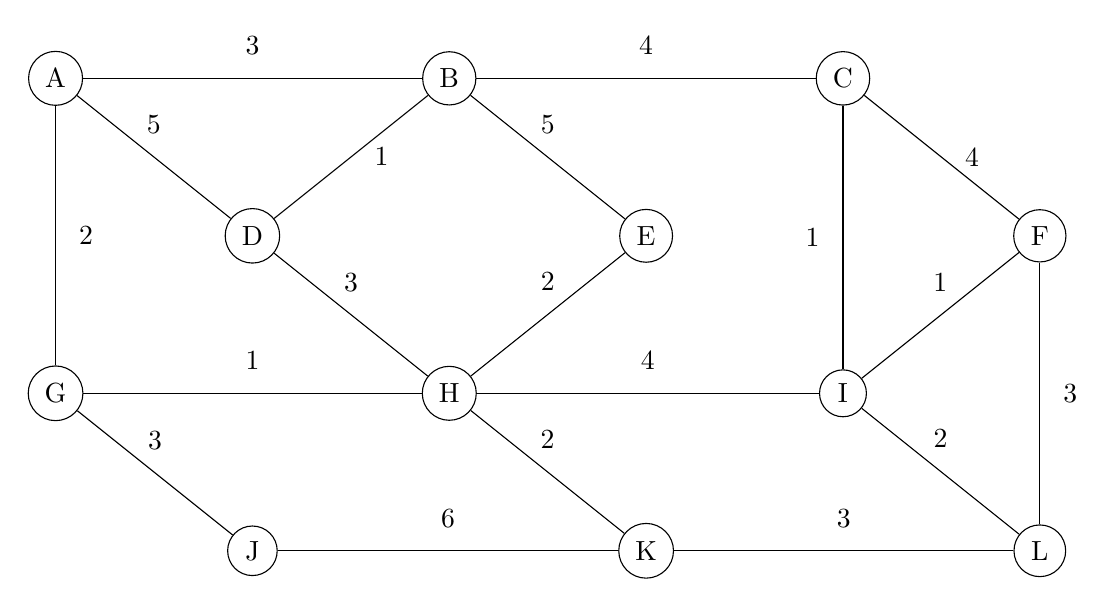
\begin{tikzpicture}
  \node[circle,draw] (va) at (0,6) {A};
  \node[circle,draw] (vb) at (5,6) {B};
  \node[circle,draw] (vc) at (10,6) {C};
  \node[circle,draw] (vd) at (2.5,4) {D};
  \node[circle,draw] (ve) at (7.5,4) {E};
  \node[circle,draw] (vf) at (12.5,4) {F};
  \node[circle,draw] (vg) at (0,2) {G};
  \node[circle,draw] (vh) at (5,2) {H};
  \node[circle,draw] (vi) at (10,2) {I};
  \node[circle,draw] (vj) at (2.5,0) {J};
  \node[circle,draw] (vk) at (7.5,0) {K};
  \node[circle,draw] (vl) at (12.5,0) {L};

  \draw (va) edge node[above=5pt] {3} (vb);
  \draw (va) edge node[above=5pt] {5} (vd);
  \draw (va) edge node[right=5pt] {2} (vg);
  \draw (vb) edge node[above=5pt] {4} (vc);
  \draw (vb) edge node[right=5pt] {1} (vd);
  \draw (vb) edge node[above=5pt] {5} (ve);
  \draw (vc) edge node[right=5pt] {4} (vf);
  \draw (vc) edge node[left=5pt] {1} (vi);
  \draw (vd) edge node[above=5pt] {3} (vh);
  \draw (ve) edge node[above=5pt] {2} (vh);
  \draw (vf) edge node[above=5pt] {1} (vi);
  \draw (vf) edge node[right=5pt] {3} (vl);
  \draw (vg) edge node[above=5pt] {1} (vh);
  \draw (vg) edge node[above=5pt] {3} (vj);
  \draw (vh) edge node[above=5pt] {4} (vi);
  \draw (vh) edge node[above=5pt] {2} (vk);
  \draw (vi) edge node[above=5pt] {2} (vl);
  \draw (vj) edge node[above=5pt] {6} (vk);
  \draw (vk) edge node[above=5pt] {3} (vl);

\end{tikzpicture}
\vskip12pt
}
\def\problemSolution{
\textcolor{blue}{
\textbf{Answer:}\\
This is what the answer should look like. Note that this is not part of a
correct answer.
\\[6pt]
\begin{tabular}{|c|c|c|c|c|c|c|c|c|c|c|c|}
  \hline
  {\bf A} & {\bf B} & {\bf C} & {\bf D} & {\bf E} & {\bf F} &
  {\bf G} & {\bf H} & {\bf I} & {\bf J} & {\bf K} & {\bf L}\\
  \hline
  \fbox{A/-/0} & B/A/3 & C/-/- & D/A/5 & E/-/- & F/-/- &
  G/A/2 & H/-/- & I/-/- & J/-/- & K/-/- & L/-/-\\
   & B/A/3 & C/-/- & D/A/5 & E/-/- & F/-/- &
  \fbox{G/A/2} & H/G/1 & I/-/- & J/G/3 & K/-/- & L/-/-\\
  \hline
\end{tabular}
}
}
\gdef\problemOutcomes{CS 2, CS 6, 5870-2}
